\section{Conformer Encoder}

Our audio encoder first processes the input with a convolution subsampling layer and then with a number of conformer blocks, as illustrated in Figure~\ref{fig:conformer}. The distinctive feature of our model is the use of Conformer blocks in the place of Transformer blocks as in~\cite{zhang2020transformer, karita2019comparative}.


A conformer block is composed of four modules stacked together, i.e, a feed-forward module, a self-attention module, a convolution module, and a second feed-forward module in the end. 
Sections~\ref{sec:model:atten}, \ref{sec:model:convolution}, and \ref{sec:model:ffn} introduce the self-attention,  convolution, and feed-forward modules, respectively. Finally, \ref{sec:model:conformer} describes how these sub blocks are combined.


\subsection{Multi-Headed Self-Attention Module}
\label{sec:model:atten}

We employ multi-headed self-attention (MHSA) while integrating an important technique from Transformer-XL \cite{dai2019transformerxl}, the relative sinusoidal positional encoding scheme. The relative positional encoding allows the self-attention module to generalize better on different input length and the resulting encoder is more robust to the variance of the utterance length. We use pre-norm residual units~\cite{wang-etal-2019-learning-deep, nguyen2019transformers} with dropout which helps training and regularizing deeper models. Figure~\ref{fig:mhsa} below illustrates the multi-headed self-attention block.

\label{sec:model:atten:selfatten}
\begin{figure}[h!]
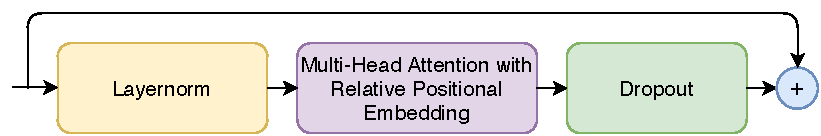
\includegraphics[width=0.9\columnwidth]{figure/mhsa.pdf}
    \caption{\textbf{Multi-Headed self-attention module.} We use multi-headed self-attention with relative positional embedding in a pre-norm residual unit.} 
    \label{fig:mhsa}
\end{figure}

\subsection{Convolution Module}
Inspired by \cite{wu2020lite}, the convolution module starts with a gating mechanism \cite{dauphin2017language}---a pointwise convolution and a gated linear unit (GLU). This is followed by a single 1-D depthwise convolution layer.
Batchnorm is deployed just after the convolution to aid training deep models. Figure~\ref{fig:conv} illustrates the convolution block.

\subsection{Feed Forward Module}
\label{sec:model:ffn}
The Transformer architecture as proposed in \cite{vaswani2017attention} deploys a feed forward module after the MHSA layer and is composed of two linear transformations and a nonlinear activation in between. A residual connection is added over the feed-forward layers, followed by layer normalization.
This structure is also adopted by Transformer ASR models~\cite{zhang2020transformer, dong2018speech}.

We follow pre-norm residual units~\cite{wang-etal-2019-learning-deep, nguyen2019transformers} and apply layer normalization within the residual unit and on the input before the first linear layer. We also apply Swish activation \cite{ramachandran2017searching} and dropout, which helps regularizing the network. Figure~\ref{fig:ffn} illustrates the Feed Forward (FFN) module.


\begin{figure*}
    \centering
    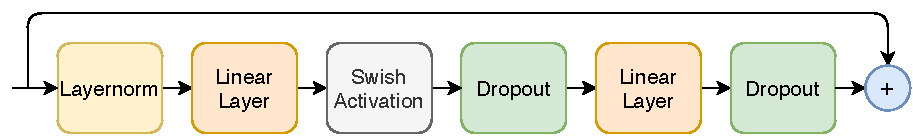
\includegraphics[width=0.5\textwidth]{figure/ffn.pdf}
    \caption{\textbf{Feed forward module.} The first linear layer uses an expansion factor of 4 and the second linear layer projects it back to the model dimension. We use swish activation and a pre-norm residual units in feed forward module.}
    \label{fig:ffn}
\end{figure*}

\subsection{Conformer Block}
\label{sec:model:conformer}
Our proposed Conformer block contains two Feed Forward modules sandwiching the Multi-Headed Self-Attention module and the Convolution module, as shown in Figure~\ref{fig:conformer}.

This sandwich structure is inspired by Macaron-Net~\cite{lu2019understanding}, which proposes  replacing the original feed-forward layer in the Transformer block into two half-step feed-forward layers, one before the attention layer and one after.  
As in Macron-Net, we employ half-step residual weights in our feed-forward (FFN) modules. The second feed-forward module is followed by a final layernorm layer.
Mathematically, this means, for input $x_{i}$ to a Conformer block $i$, the output $y_{i}$ of the block is:
\begin{equation}
\begin{split}
    \tilde{x_{i}}&= x_{i} + \frac{1}{2}\mathrm{FFN}(x_{i})    \\
    x'_{i}&= \tilde{x_{i}} + \mathrm{MHSA}(\tilde{x_{i}})    \\
    x''_{i}&= x'_{i} + \mathrm{Conv}(x'_{i})    \\
    y_{i}&= \mathrm{Layernorm}(x''_{i} + \frac{1}{2}\mathrm{FFN}(x''_{i}))    \\
\end{split}
\label{model:conformer:equation}
\end{equation}
where FFN refers to the Feed forward module, MHSA refers to the Multi-Head Self-Attention module, and Conv refers to the Convolution module as described in the preceding sections.

Our ablation study discussed in Sec~\ref{ablate_conformer_macaron} compares the Macaron-style half-step FFNs with the vanilla FFN as used in previous works. We find that having two Macaron-net style feed-forward layers with half-step residual connections sandwiching the attention and convolution modules in between provides a significant improvement over having a single feed-forward module in our Conformer architecture.

The combination of convolution and self-attention has been studied before and one can imagine many ways to achieve that. 
Different options of augmenting convolutions with self-attention are studied in Sec~\ref{ablate_conformer_convolution}.
We found that convolution module stacked after the self-attention module works best for speech recognition.